\documentclass{beamer}
\usepackage[utf8]{inputenc}

\usetheme{Madrid}
\usecolortheme{default}
\usepackage{amsmath,amssymb,amsfonts,amsthm}
\usepackage{txfonts}
\usepackage{tkz-euclide}
\usepackage{listings}
\usepackage{adjustbox}
\usepackage{array}
\usepackage{tabularx}
\usepackage{gvv}
\usepackage{lmodern}
\usepackage{circuitikz}
\usepackage{tikz}
\usepackage{graphicx}
\usepackage{mathtools}

\setbeamertemplate{page number in head/foot}[totalframenumber]

\usepackage{tcolorbox}
\tcbuselibrary{minted,breakable,xparse,skins}



\definecolor{bg}{gray}{0.95}
\DeclareTCBListing{mintedbox}{O{}m!O{}}{%
  breakable=true,
  listing engine=minted,
  listing only,
  minted language=#2,
  minted style=default,
  minted options={%
    linenos,
    gobble=0,
    breaklines=true,
    breakafter=,,
    fontsize=\small,
    numbersep=8pt,
    #1},
  boxsep=0pt,
  left skip=0pt,
  right skip=0pt,
  left=25pt,
  right=0pt,
  top=3pt,
  bottom=3pt,
  arc=5pt,
  leftrule=0pt,
  rightrule=0pt,
  bottomrule=2pt,
  toprule=2pt,
  colback=bg,
  colframe=orange!70,
  enhanced,
  overlay={%
    \begin{tcbclipinterior}
    \fill[orange!20!white] (frame.south west) rectangle ([xshift=20pt]frame.north west);
    \end{tcbclipinterior}},
  #3,
}
\lstset{
    language=C,
    basicstyle=\ttfamily\small,
    keywordstyle=\color{blue},
    stringstyle=\color{orange},
    commentstyle=\color{green!60!black},
    numbers=left,
    numberstyle=\tiny\color{gray},
    breaklines=true,
    showstringspaces=false,
}
\title{4.11.23}
\date{26th September, 2025}
\author{Puni Aditya - EE25BTECH11046}

\begin{document}

\frame{\titlepage}
\begin{frame}{Question}
Find the co-ordinates of the point where the line $\frac{x-3}{-1} = \frac{y+4}{1} = \frac{z+5}{6}$ crosses the plane passing through the points $\brak{\frac{7}{2}, 0, 0}$, $\brak{0, 7, 0}$, and $\brak{0, 0, 7}$.
\end{frame}

\begin{frame}{Theoretical Solution}
For the intersection of a line
\begin{align*}
    \vec{x} = \vec{p} + \lambda\vec{m}
\end{align*}    
with the plane
\begin{align*}
    \vec{n}^\top\vec{x} = c
\end{align*}
\begin{align}
    \vec{n}^\top\brak{\vec{p}+\lambda\vec{m}} &= c \\
    \vec{n}^\top\vec{p} + \lambda\vec{n}^\top\vec{m} &= c \\
    \lambda &= \frac{c - \vec{n}^\top\vec{p}}{\vec{n}^\top\vec{m}} \label{eq:27} \\
    \vec{x} &= \vec{p} + \brak{\frac{c - \vec{n}^\top\vec{p}}{\vec{n}^\top\vec{m}}}\vec{m} \label{eq:28}
\end{align}
\end{frame}

\begin{frame}{Theoretical Solution}
Let the equation of the plane be 
\begin{align}
\myvec{n_1 & n_2 & n_3}\vec{x} = c \label{eq:1}
\end{align}
The three points 
\begin{align*}
    \vec{P_1} = \myvec{\frac{7}{2} \\ 0 \\ 0}, \vec{P_2} = \myvec{0 \\ 7 \\ 0}, \vec{P_3} = \myvec{0 \\ 0 \\ 7}
\end{align*}
satisfy this equation, giving the system:
\begin{align}
    \frac{7}{2}n_1 + 0n_2 + 0n_3 &= c \\
    0n_1 + 7n_2 + 0n_3 &= c \\
    0n_1 + 0n_2 + 7n_3 &= c
\end{align}
\end{frame}

\begin{frame}{Theoretical Solution}
This system of equations gives the augmented matrix
\begin{align}
    \myaugvec{3}{
        \frac{7}{2} & 0 & 0 & c \\
        0 & 7 & 0 & c \\
        0 & 0 & 7 & c
    }
    \xleftrightarrow[\text{R}_3 \to \frac{1}{7}\text{R}_3]{\text{R}_1 \to \frac{2}{7}\text{R}_1, \text{R}_2 \to \frac{1}{7}\text{R}_2}
    \myaugvec{3}{
        1 & 0 & 0 & \frac{2c}{7} \\
        0 & 1 & 0 & \frac{c}{7} \\
        0 & 0 & 1 & \frac{c}{7}
    }
\end{align}
From the row-reduced echelon form,
\begin{align}
    n_1 = \frac{2c}{7}, n_2 = \frac{c}{7}, n_3 = \frac{c}{7} \label{eq:2}
\end{align}
\end{frame}

\begin{frame}{Theoretical Solution}
Substituting \eqref{eq:2} in \eqref{eq:1},
\begin{align}
    \myvec{\frac{2c}{7} & \frac{c}{7} & \frac{c}{7}}\vec{x} = c
\end{align}
Assuming $c \neq 0$, the equation simplifies to the normal form of the plane, $\vec{n}^\top\vec{x} = c$, which is
\begin{align}
    \myvec{2 & 1 & 1}\vec{x} = 7 \label{eq:plane_eqn}
\end{align}
\end{frame}

\begin{frame}{Theoretical Solution}
The vector equation of the line passing through 
\begin{align*}
\vec{p} = \myvec{3 \\ -4 \\ -5}
\end{align*}
with direction vector 
\begin{align*}
    \vec{m} = \myvec{-1 \\ 1 \\ 6}
\end{align*}
is
\begin{align}
    \vec{x} = \myvec{3 \\ -4 \\ -5} + \lambda \myvec{-1 \\ 1 \\ 6} \label{eq:line_eqn}
\end{align}
\end{frame}

\begin{frame}{Theoretical Solution}
Using \eqref{eq:28},
\begin{align}
    \vec{x} &= \myvec{3 \\ -4 \\ -5} + \brak{\frac{7 - \myvec{2 & 1 & 1}\myvec{3 \\ -4 \\ -5}}{\myvec{2 & 1 & 1}\myvec{-1 \\ 1 \\ 6}}}\myvec{-1 \\ 1 \\ 6} \\
    \vec{x} &= \myvec{3 \\ -4 \\ -5} + 2\myvec{-1 \\ 1 \\ 6} = \myvec{1 \\ -2 \\ 7}
\end{align}
The co-ordinates of the point of intersection are $\myvec{1 \\ -2 \\ 7}$.
\end{frame}

\begin{frame}{Plot}
    \begin{figure}
        \centering
        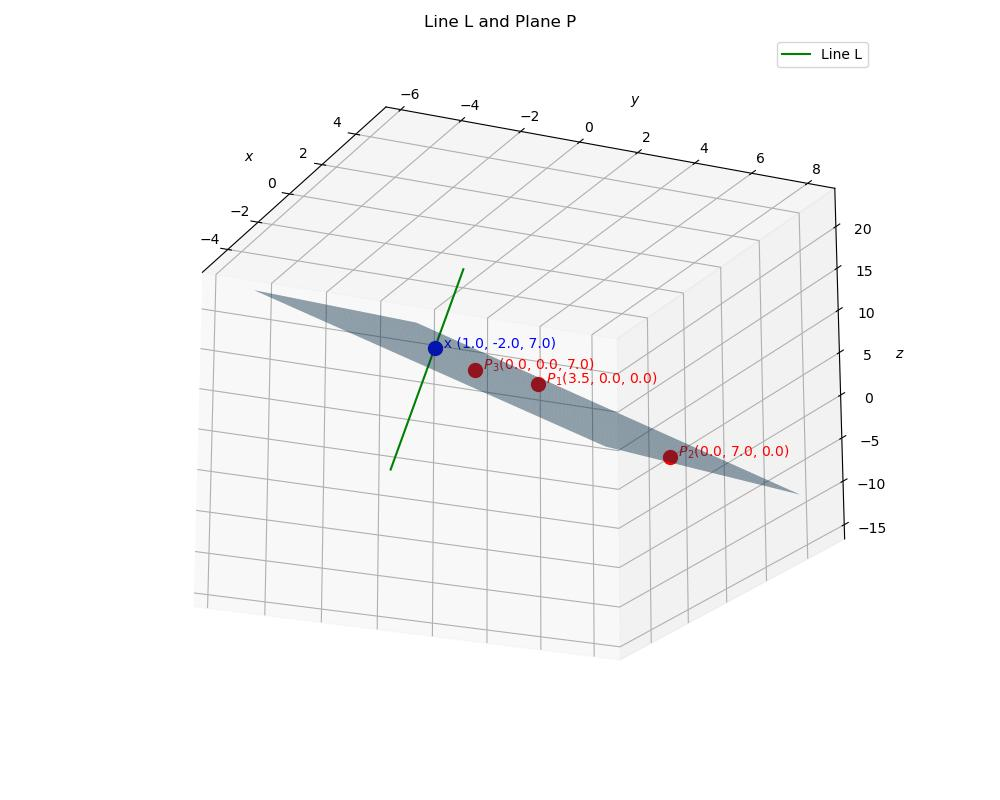
\includegraphics[width=0.7\columnwidth]{../figs/plot_c.jpg}
        \caption{Plot}
        \label{fig:fig}
    \end{figure}
\end{frame}

\end{document}
